% ch10b Bosonization, part b (书页 162-168 / 分册p017-023)
%--TAIL--
因子 4 来源于每个电子的两项空穴子–自旋子（holon–spinon）相互作用，再加上两个电子之间的交叉相互作用。我们已假定单态中自旋子的能量为零。这两个态的能量差为
\begin{equation*}
E_{\mathrm{pair}}^{(1)}=-\left(2V_{\mathrm{hs}}+V_{\mathrm{hh}}+V_{\mathrm{ss}}\right),
\tag{10.68}
\end{equation*}
要使单个电子稳定，须有 $V_{\mathrm{hs}}<0$；而库仑定律规定 $V_{\mathrm{hh}}>0$。于是，自旋子–自旋子相互作用能便是决定 $E_{\mathrm{pair}}^{(1)}\lessgtr 0$ 的关键量。在某些情形下，$V_{\mathrm{ss}}$ 恰好具有合适的量值，使得 $E_{\mathrm{pair}}^{(1)}>0$。此时，纯粹排斥性的电子相互作用也能导致配对结合。

\section{激发谱}

如果将式 (10.63) 与谐振子的标准哈密顿量 $H=P^{2}+Q^{2}$（其中 $P$ 与 $Q$ 为正则动量与坐标）相比较，就会发现玻色化后的电荷部分与一群谐振子等价。正如前文所指出的，卢廷格模型中的电荷激发就是通常的玻色模式，更为人熟知的名称是等离激元激发。这些激发相应的态密度应当是什么？人们或许猜想它们服从标准的玻色–爱因斯坦分布，然而事实并非如此。卢廷格液体（L1960）中的电荷激发，其态密度在费米能级处按 $|k-k_{\mathrm{F}}|^{\alpha}$ 的形式消失，这完全来源于电子之间的关联。该幂律由 $\alpha=(g_{\mathrm{c}}+g_{\mathrm{c}}^{-1})/2-1$ 给出。因此，卢廷格液体并不具有标志费米液体特征的光滑态密度，而是对任何 $U\neq0$ 都会在费米能级处发展出一个软能隙（soft gap）。这一效应的根源可以追溯到电子气的玻色化形式中 $v_{\mathrm{F}}^{\mathrm{c}}$ 被 $g_{\mathrm{c}}$ 重正化。

我们通过计算总电荷关联函数来确立这一结果：
\begin{equation*}
G(x)=\left\langle\sum_{\sigma}\left(\Psi_{\sigma+}(x)\Psi_{\sigma+}^{\dagger}(0)+\Psi_{\sigma-}(x)\Psi_{\sigma-}^{\dagger}(0)\right)\right\rangle.
\tag{10.69}
\end{equation*}
为使记号紧凑，我们定义
\begin{equation*}
\Theta_{\sigma}(x)=\int_{-\infty}^{x}\Pi_{\sigma}(x')\,\mathrm{d}x'.
\tag{10.70}
\end{equation*}

对每个自旋分量，我们作代换 $\Phi_{\uparrow(\downarrow)}=(\Phi_{\mathrm{c}}\pm\Phi_{\mathrm{s}})/\sqrt{2}$ 与 $\Theta_{\uparrow(\downarrow)}=(\Theta_{\mathrm{c}}\pm\Theta_{\mathrm{s}})/\sqrt{2}$，其中上面的符号对应自旋向上，下面的符号对应自旋向下。在没有磁场时，$n_{\uparrow}(x)=n_{\downarrow}(x)$，因而所有对 $\Phi_{\mathrm{s}}$ 或 $\Pi_{\mathrm{s}}$ 线性的平均恒等于零。利用变换后的场 $\tilde{\Phi}_{\nu}(x)$ 与 $\tilde{\Pi}_{\nu}(x)$，我们可以把式 (10.69) 中的平均进一步化简。此时，式 (10.69) 中的平均是对以重正化费米速度 $v_{\mathrm{F}}^{\mathrm{c}}$ 与 $v_{\mathrm{F}}^{\mathrm{s}}$ 为特征的非相互作用玻色化系统的基态取的。于是可以使用化简玻色算符指数函数乘积平均的标准规则。利用 Baker–Hausdorff 恒等式的第三种形式（式 (10.48)），我们发现总电子密度的关联函数化简为
\begin{equation*}
G(x)=\frac{1}{\pi a}\,\mathrm{e}^{\mathrm{i}\,\text{相位}}\,\mathrm{e}^{\frac{\pi}{2}\sum_{\nu=\mathrm{c},\mathrm{s}}\left(g_{\nu}^{-1}a_{\nu}+g_{\nu}b_{\nu}\right)},
\tag{10.71}
\end{equation*}
其中
\begin{equation*}
a_{\nu}=\langle\tilde{\Phi}_{\nu}(x)\tilde{\Phi}_{\nu}(0)-\tilde{\Phi}_{\nu}^{2}(0)\rangle
\tag{10.72}
\end{equation*}
且
\begin{equation*}
b_{\nu}=\langle\tilde{\Theta}_{\nu}(x)\tilde{\Theta}_{\nu}(0)-\tilde{\Theta}_{\nu}^{2}(0)\rangle.
\tag{10.73}
\end{equation*}
相位由交叉项决定。对电荷场与自旋场，交叉项都具有 $\langle\tilde{\Phi}_{\nu}(0)\tilde{\Theta}_{\nu}(0)+\tilde{\Theta}_{\nu}(0)\tilde{\Phi}_{\nu}(0)\rangle-\langle\tilde{\Phi}_{\nu}(x)\tilde{\Theta}_{\nu}(0)+\tilde{\Theta}_{\nu}(x)\tilde{\Phi}_{\nu}(0)\rangle$ 的形式。这一项恒为零（见习题 10.4）。

计算 $G(x)$ 中各平均的最简单办法是引入自由玻色场的傅里叶展开\footnote{译注：原书式 (10.74) 中两处算符的宗量印作 $\phi_{\nu}(x)$，按式 (10.75) 的对易关系应为 $\phi_{\nu}(p)$，此处已按本意改正。}：
\begin{align*}
\tilde{\Phi}_{\nu}(x)&=\int_{-\infty}^{\infty}\frac{\mathrm{d}p}{2\pi\sqrt{2|p|}}\,\mathrm{e}^{-a|p|/2}\left[\phi_{\nu}(p)\,\mathrm{e}^{\mathrm{i}px}+\phi_{\nu}^{\dagger}(p)\,\mathrm{e}^{-\mathrm{i}px}\right],\\
\tilde{\Pi}_{\nu}(x)&=\int_{-\infty}^{\infty}\frac{\mathrm{d}p\,|p|}{2\pi\sqrt{2|p|}}\,\mathrm{e}^{-a|p|/2}\left[-\mathrm{i}\phi_{\nu}(p)\,\mathrm{e}^{\mathrm{i}px}+\mathrm{i}\phi_{\nu}^{\dagger}(p)\,\mathrm{e}^{-\mathrm{i}px}\right],
\tag{10.74}
\end{align*}
其中
\begin{equation*}
\left[\phi_{\nu}(p),\phi_{\nu}^{\dagger}(q)\right]=2\pi\delta(q-p)
\tag{10.75}
\end{equation*}
且 $\nu=\mathrm{c},\mathrm{s}$。由这些表达式可得
\begin{equation*}
\langle\tilde{\Phi}_{\nu}(x)\tilde{\Phi}_{\nu}(0)-\tilde{\Phi}_{\nu}^{2}(0)\rangle=\frac{1}{4\pi}\ln\left(\frac{a^{2}}{a^{2}+x^{2}}\right).
\tag{10.76}
\end{equation*}

对于共轭场，类似结果的推导要复杂一些，因此我们显式地完成这一计算。由 $\tilde{\Theta}(x)$ 的定义，可将 $\tilde{\Theta}_{\nu}(x)$ 的关联函数化为
\begin{equation*}
\langle\tilde{\Theta}_{\nu}(x)\tilde{\Theta}_{\nu}(0)-\tilde{\Theta}_{\nu}^{2}(0)\rangle=\int_{0}^{x}\mathrm{d}x'\int_{-\infty}^{0}\mathrm{d}x''\,\langle\tilde{\Pi}_{\nu}(x')\tilde{\Pi}_{\nu}(x'')\rangle.
\tag{10.77}
\end{equation*}
为化简对共轭动量场的平均，注意到 $\langle\phi_{\nu}(p)\phi_{\nu}^{\dagger}(q)\rangle=2\pi\delta(p-q)$。于是
\begin{align*}
\langle\tilde{\Pi}_{\nu}(x')\tilde{\Pi}_{\nu}(x'')\rangle&=\int_{-\infty}^{\infty}\frac{\mathrm{d}p\,|p|}{4\pi}\,\mathrm{e}^{\mathrm{i}p(x'-x'')}\,\mathrm{e}^{-a|p|}\\
&=\frac{-1}{2\pi}\left[\frac{(x'-x'')^{2}-a^{2}}{\left(a^{2}+(x'-x'')^{2}\right)^{2}}\right].
\tag{10.78}
\end{align*}
将此式代入式 (10.77)，得到
\begin{align*}
\langle\tilde{\Theta}_{\nu}(x)\tilde{\Theta}_{\nu}(0)-\tilde{\Theta}_{\nu}^{2}(0)\rangle&=\frac{1}{2\pi}\int_{0}^{x}\mathrm{d}x'\int_{-\infty}^{x'}\mathrm{d}y\,\frac{y^{2}-a^{2}}{(a^{2}+y^{2})^{2}}\\
&=\frac{-1}{2\pi}\int_{0}^{x}\mathrm{d}x'\,\frac{y}{a^{2}+y^{2}}\\
&=\frac{1}{4\pi}\ln\frac{a^{2}}{a^{2}+x^{2}}
\tag{10.79}
\end{align*}

于是，总电子密度的关联函数（式 (10.71)）
\begin{equation*}
G(x)\propto|x|^{-\frac{g_{\mathrm{c}}+g_{\mathrm{c}}^{-1}+g_{\mathrm{s}}+g_{\mathrm{s}}^{-1}}{4}}
\tag{10.80}
\end{equation*}
随距离作代数式衰减。电子关联函数的代数式衰减是一维关联电子系统的关键定义特征。围绕 $k_{\mathrm{F}}$ 的动量分布函数通过傅里叶变换定义：
\begin{align*}
n(k)&=\int_{-\frac{L}{2}}^{\frac{L}{2}}\mathrm{d}x\,\mathrm{e}^{\mathrm{i}(k-k_{\mathrm{F}})x}\,G(x)\\
&\propto\int_{-\frac{L}{2}}^{\frac{L}{2}}\mathrm{d}x\,\mathrm{e}^{\mathrm{i}(k-k_{\mathrm{F}})x}\,|x|^{-\frac{g_{\mathrm{c}}+g_{\mathrm{c}}^{-1}+g_{\mathrm{s}}+g_{\mathrm{s}}^{-1}}{4}}.
\tag{10.81}
\end{align*}
作变量代换 $y=(k-k_{\mathrm{F}})x$ 后，我们发现电子激发的动量分布函数
\begin{equation*}
n(k)\propto\left|k-k_{\mathrm{F}}\right|^{\frac{g_{\mathrm{c}}+g_{\mathrm{c}}^{-1}+g_{\mathrm{s}}+g_{\mathrm{s}}^{-1}}{4}-1},
\tag{10.82}
\end{equation*}
在费米能级附近代数式地趋于零，如图 10.5 所示。对于无自旋电子，由变换到电荷场与自旋场所产生的 $1/\sqrt{2}$ 因子不会出现，结果式 (10.71) 指数中的因子 $\pi/2$ 被换成 $\pi$。因此，无自旋电子情形相应的指数为 $(g_{\mathrm{c}}+g_{\mathrm{c}}^{-1})/2-1$。然而，在两种情形下，只要令 $g_{\nu}=1$，我们就回到费米液体的条件，即态密度在费米能级处为非零常数。分布函数在费米能级处的代数式消失表明：与费米液体不同，卢廷格液体中不存在良好定义的准粒子。低温下 $k-k_{\mathrm{F}}$ 的特征值由 $|k^{2}/2m-k_{\mathrm{F}}^{2}/2m|\sim|k-k_{\mathrm{F}}|v_{\mathrm{F}}\sim T$ 给出。于是，动量分布函数在费米能级处的代数式消失转化为激发谱具有如下形式的代数式温度依赖
\begin{equation*}
n(T)\propto T^{\frac{g_{\mathrm{c}}+g_{\mathrm{c}}^{-1}}{2}-1}
\tag{10.83}
\end{equation*}

\begin{figure}[H]\centering
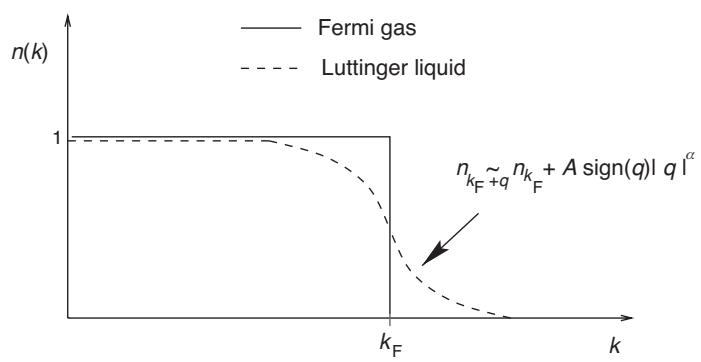
\includegraphics[width=0.62\textwidth]{figs/ch10/fig_10.5_a.jpg}\\[0.8ex]
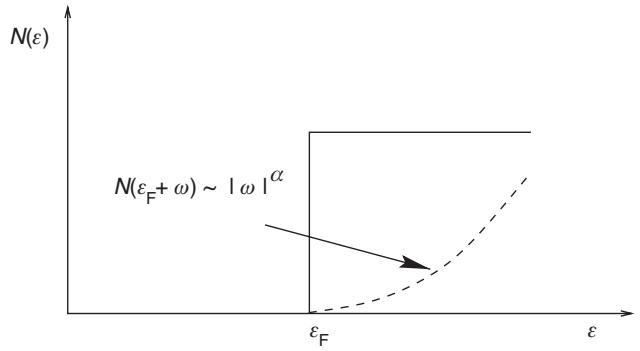
\includegraphics[width=0.60\textwidth]{figs/ch10/fig_10.5_b.jpg}
\caption*{图 10.5\quad 图中给出卢廷格液体（虚线）与费米气体（实线）的动量分布（上图）与隧穿态密度（下图）。图中展示了动量分布函数在费米能量附近的特征性代数依赖。在费米气体极限下，$\alpha=0$，且常数 $A=-1/2$。隧穿态密度在费米能级处消失，正是图 10.6 所示 $I$–$V$ 特性代数式温度依赖的根源。}\label{fig:auto:10.5}
\end{figure}

这样的代数标度预计会产生深刻的实验后果。考虑一个隧穿实验，其中电子越过势垒进入卢廷格液体。通过任何系统的输运都由载流子可资利用的电子态的分布决定。因此可以预期，当 $T\to0$ 时，跨过分隔两个卢廷格液体的势垒的电导（透射率）将趋于零。于是，电导不应以特征激活能的形式随偏离 $T=0$ 而指数式增大，而应以幂律增大（KF1992）。这一幂律应当出现在卢廷格液体输运的电流–电压（$I$–$V$）特性测量中。Chang 及其合作者（CPW1996）在表现出卢廷格液体行为的体系中完成了展示 $I$–$V$ 特性幂律依赖的实验，其数据如图 10.6 所示。在这些特定的实验中，卢廷格液体是分数量子霍尔效应态的边缘态。对于这些样品，Kane 和 Fisher（KF1992）证明电流按如下方式标度：
\begin{equation*}
I\propto T^{\alpha}\left[x+x^{\alpha}\right]
\tag{10.84}
\end{equation*}
其中 $\alpha=3$，$x=eV/2\pi k_{\mathrm{F}}T$。取 $\alpha=2.7$ 以及电压与温度之间的 $1/2\pi$ 标度因子，理论取得了与实验极好的符合。Webb 及其合作者（MUW1996）在量子霍尔体系中，以及 Bockrath 及其同事（B1999）在碳纳米管上也得到了类似结果。由此可见，电子关联是一维电子体系电流–电压特性幂律依赖的核心，这一点已有坚实的实验基础。

\begin{figure}[H]\centering
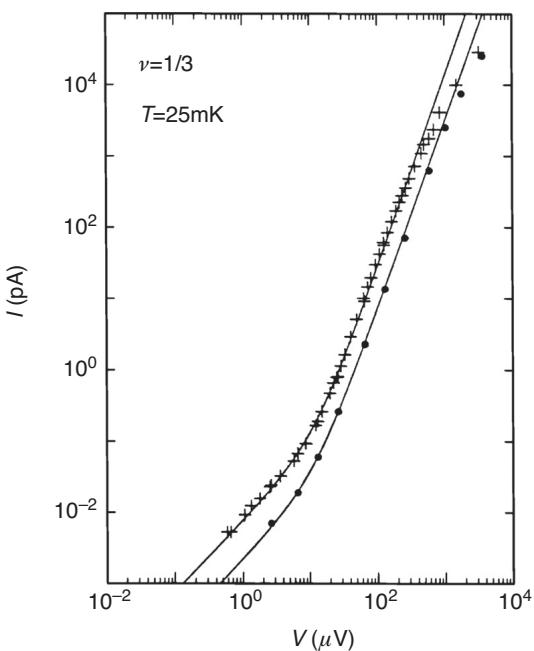
\includegraphics[width=0.48\textwidth]{figs/ch10/fig_10.6.jpg}
\caption*{图 10.6\quad 从体掺杂 $n^{+}$\,GaAs 隧穿进入最低朗道能级填充因子为 $\nu=1/3$ 的分数量子霍尔效应态边缘时的电流–电压（$I$–$V$）特性。实心圆点与十字分别对应磁场 $B=10.8\,\mathrm{T}$ 与 $B=13.4\,\mathrm{T}$。分数量子霍尔态中的边缘态是卢廷格液体。由于隧穿态密度的代数式依赖（见式 (10.82)），隧穿进入卢廷格液体时 $I$ 随 $V$ 预期呈代数式依赖。实曲线是对理论普适形式（式 (10.84)）的拟合。}\label{fig:auto:10.6}
\end{figure}

在本章收尾之际，我们简要评论一下：在半满时保留 Umklapp 项会发生什么。此时电荷部分出现一个余弦项，这意味着在半满时，对排斥相互作用而言电荷部分存在激发能隙。这表明空穴子若不付出巨大的能量代价便不能自由地导电。出现这种情形是因为半满时每个格点上恰好有一个电子，因此把一个电子从一个格点移动到另一个格点的能量代价为 $U$，即电荷能隙的大小。

若 $U$ 为负，则半满时的基态将是每个格点上两个紧紧束缚在一起的电子（结合能量级为 $U$）。这样的实体移动时无需耗费能量。因此，在半满时，只有排斥相互作用才存在电荷能隙。

\section*{小结}
\addcontentsline{toc}{section}{小结}

在一维情形，对存在短程相互作用的电子气，可以发展出一幅关于其集体激发的玻色化图像。这一描述层次使我们能够清晰地证明：一维中自旋与电荷以根本不同的速度运动。至于自旋–电荷分离在 $d>1$ 时如何严格地建立，目前仍属未知。此外，一维中的库仑相互作用导致态密度在费米能级处代数式衰减。态密度的这种特征性衰减是卢廷格液体行为的标志，并且可以在隧穿实验中观测到。某些情形可能需要超出线性近似的物理，那时就必须推广这里介绍的玻色化方法。

\section*{习题}
\addcontentsline{toc}{section}{习题}

\textbf{习题 10.1}\quad 证明：若把式 (10.31) 代入哈密顿量的连续版本（式 (10.6)），所得的玻色哈密顿量将对应于式 (10.30) 的两倍。

\textbf{习题 10.2}\quad 利用式 (10.43) 与 Baker–Hausdorff 恒等式（式 (10.38)）证明
\begin{equation*}
:\mathrm{e}^{\mathcal{A}}::\mathrm{e}^{\mathcal{B}}:=:\mathrm{e}^{\mathcal{A}+\mathcal{B}}:\,\mathrm{e}^{[\mathcal{A}^{-},\mathcal{B}^{+}]}.
\tag{10.85}
\end{equation*}

\textbf{习题 10.3}\quad 证明电流各分量之间的等时对易关系由下式给出：
\begin{equation*}
\left[j_{0}^{\sigma}(x),j_{1}^{\sigma}(y)\right]=-\frac{\mathrm{i}\hbar v_{\mathrm{F}}}{\pi}\partial_{x}\delta(x-y),
\tag{10.86}
\end{equation*}
\begin{equation*}
\left[j_{0}^{\sigma}(x),j_{0}^{\sigma}(y)\right]=\left[j_{1}^{\sigma}(x),j_{1}^{\sigma}(y)\right]=0.
\tag{10.87}
\end{equation*}

\textbf{习题 10.4}\quad 证明式 (10.71) 中的相位因子恒为零。你也许会发现下述攻略有所帮助。首先注意 $\Theta_{\nu}$ 与 $\Phi_{\nu}$ 相对 $g_{\nu}$ 的标度互为倒数，因此各交叉项与重标度因子无关。由连续性方程 $\partial_{\tau}\Phi=\partial_{x}\theta$，你可以确立
\begin{equation*}
\theta(x,\tau)=\int_{-\infty}^{x}\mathrm{d}x'\,\partial_{\tau}\phi(x',\tau)
\tag{10.88}
\end{equation*}
进而确立
\begin{align*}
\langle\tilde{\Phi}_{\nu}(x,\tau)\tilde{\Theta}_{\nu}(0)-\tilde{\Theta}_{\nu}(0)\tilde{\Phi}_{\nu}(0)\rangle&=-\int_{\infty}^{x}\mathrm{d}x'\left\{\partial_{\tau}G(x,x',\tau,0)|_{\tau=0}\right.\\
&\qquad\left.-\partial_{\tau}G(0,x',\tau)|_{x'=0,\tau=0}\right\},
\tag{10.89}
\end{align*}
其中 $G(x,x',\tau,\tau')=\langle\Phi_{\nu}(x,0)\Phi_{\nu}(x',\tau)\rangle$\,\footnote{译注：原书式 (10.89) 的积分下限印作 $\infty$；按式 (10.70) 的定义，此处疑应为 $-\infty$，今照原书排印。}。随后你应能证明余下的贡献以相反的符号进入，因而总和为零。

\textbf{习题 10.5}\quad 计算能级间距为 $\epsilon$ 的无相互作用费米气体的配分函数（取费米海为无限深）。一条求解路径是证明：能量为 $N\epsilon$ 的态，其简并度等于 $N$ 的整数分拆数 $p(N)$（例如 $p(3)=3$，因为 $3=3$、$2+1$、$1+1+1$）。该配分函数对应于什么样的玻色系统？

\textbf{习题 10.6}\quad 推导式 (10.20)。

\section*{参考文献}
\addcontentsline{toc}{section}{参考文献}

\begin{itemize}[leftmargin=2em,itemsep=0pt,parsep=0pt,label={}]
\item [B1999] M. Bockrath, D. H. Cobden, L. Jia, A. G. Rinzler, R. E. Smalley, L. Balents, and P. L. McEuen, \emph{Nature (London)} \textbf{397}, 598 (1999).
\item [BP1953] D. Bohm and D. Pines, \emph{Phys. Rev.} \textbf{92}, 609 (1953).
\item [CPW1996] A. Chang, L. Pfeiffer, and K. West, \emph{Phys. Rev. Lett.} \textbf{77}, 2538 (1996).
\item [H1981] F. D. M. Haldane, \emph{J. Phys. C: Sol. State Phys.} \textbf{14}, 2585 (1981).
\item [H1964] J. Hubbard, \emph{Proc. Roy. Soc. A} \textbf{277}, 237 and 281 (1964).
\item [KF1992] C. L. Kane and M. P. A. Fisher, \emph{Phys. Rev. Lett.} \textbf{68}, 1220 (1992).
\item [KS1996] G. Kotliar and Q. Si, \emph{Phys. Rev. B} \textbf{53} (1996).
\item [L1960] J. M. Luttinger, \emph{Phys. Rev.} \textbf{119}, 1153 (1960).
\item [M1975] S. Mandelstam, \emph{Phys. Rev. D} \textbf{11}, 3026 (1975).
\item [M1974] D. Mattis, \emph{J. Math. Phys. (N.Y.)} \textbf{15}, 609 (1974).
\item [ML1965] D. Mattis and E. Lieb, \emph{J. Math. Phys.} \textbf{6}, 304 (1965).
\item [MUW1996] F. P. Milliken, C. P. Umbach, and R. A. Webb, \emph{Solid State Commun.} \textbf{97}, 309 (1996).
\item [S1990] H. J. Schulz, \emph{Phys. Rev. Lett.} \textbf{64}, 2831 (1990).
\item [S1959] J. Schwinger, \emph{Phys. Rev. Lett.} \textbf{3}, 296 (1959).
\item [T1950] S. Tomonaga, \emph{Prog. Theor. Phys. (Kyoto)} \textbf{5}, 544 (1950).
\item [VDS1998] J. von Delft and H. Schoeller, \emph{Annalen Phys.} \textbf{7}, 225 (1998).
\item [Y2005] A. Yacoby, \emph{Les Houches Summer School Proceedings} \textbf{81}, 605 (2005).
\end{itemize}
